\label{Evaluation}

In order to evaluate the performance of both alorithms, we decided to implemented them in C++ using the Boost Graph Library's (BGL) \footnote{\url{https://www.boost.org/doc/libs/1_82_0/libs/graph/doc/index.html}} graph data structure. This allowed us to easily generate random graph instances and to use the BGL's built-in functions to visualize the graphs and the k-cores. Moreover, having the both algorithms implemented in the same language and using the same graph data structure allowed us to compare them in a fair way.

\begin{figure}[H]
    \centering
    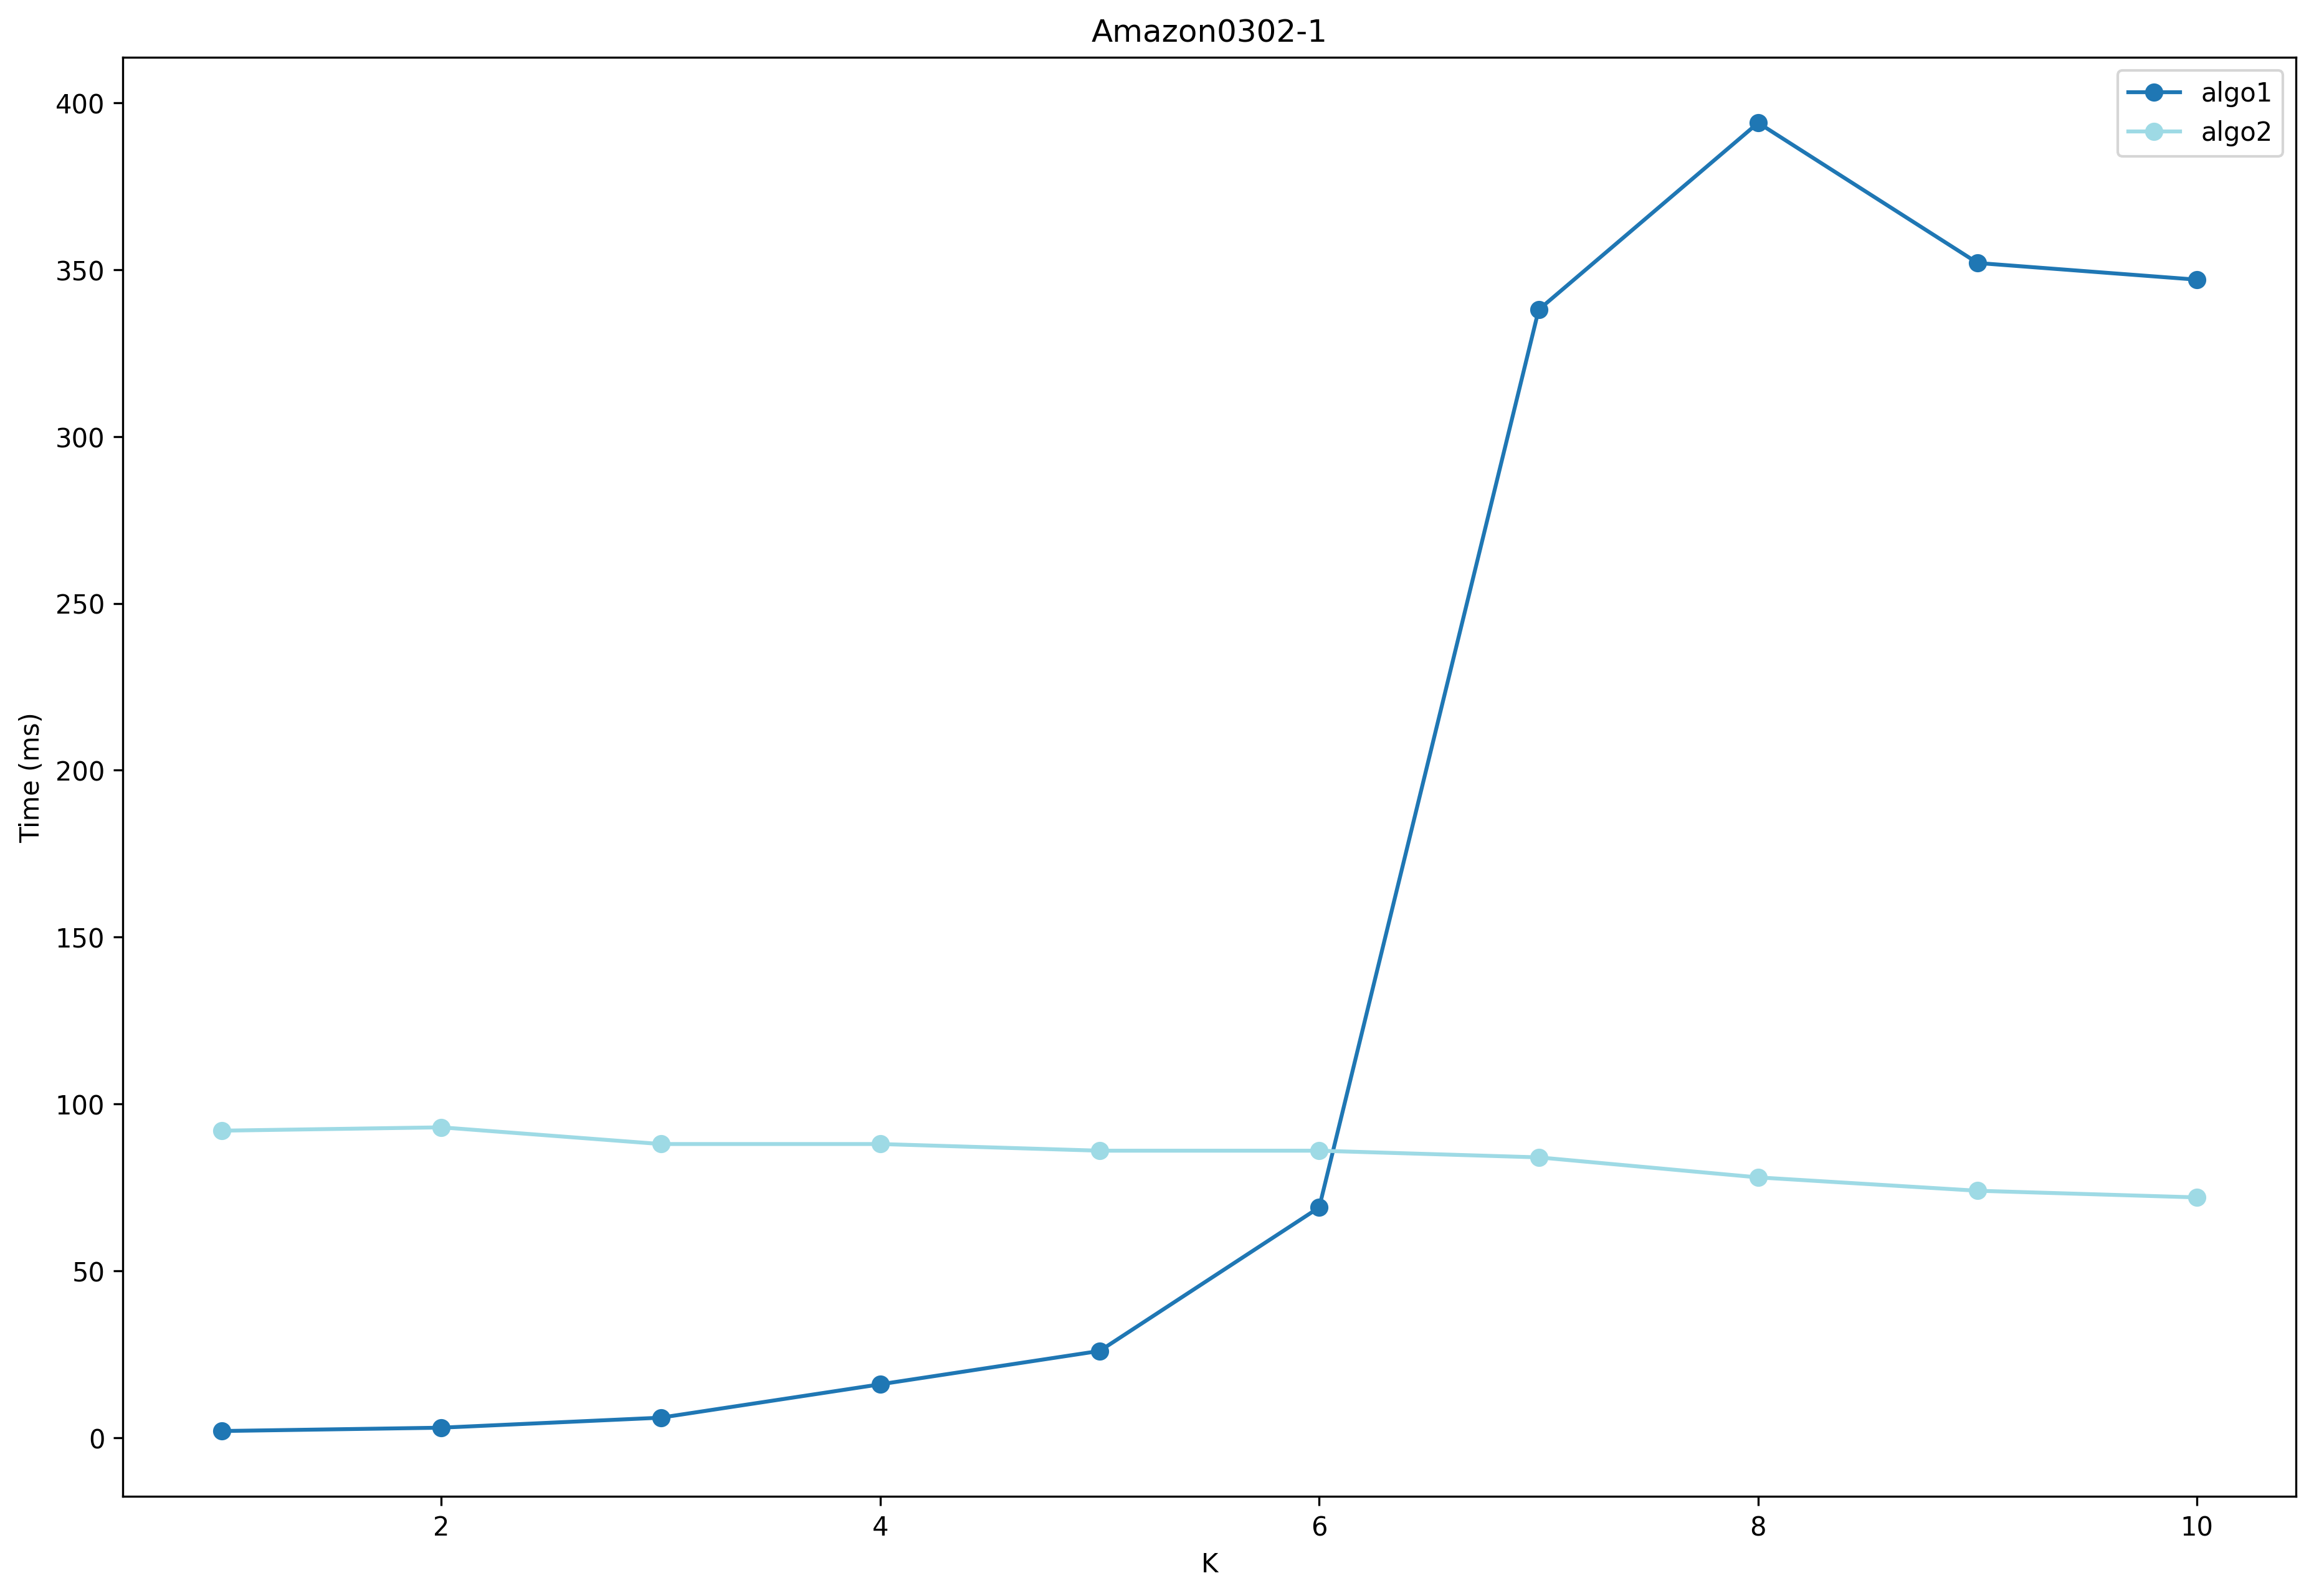
\includegraphics[width=0.6\textwidth]{Figures/Amazon0302-1.png}
    \caption{Amazon0302 benchmark times for both algorithms}
    \label{fig:amazon}
\end{figure}

\begin{figure}[H]
    \centering
    \includegraphics[width=0.6\textwidth]{Figures/cit-Patents.png}
    \caption{cit-Patents benchmark times for both algorithms}
    \label{fig:cit-patents}
\end{figure}

\begin{figure}[H]
    \centering
    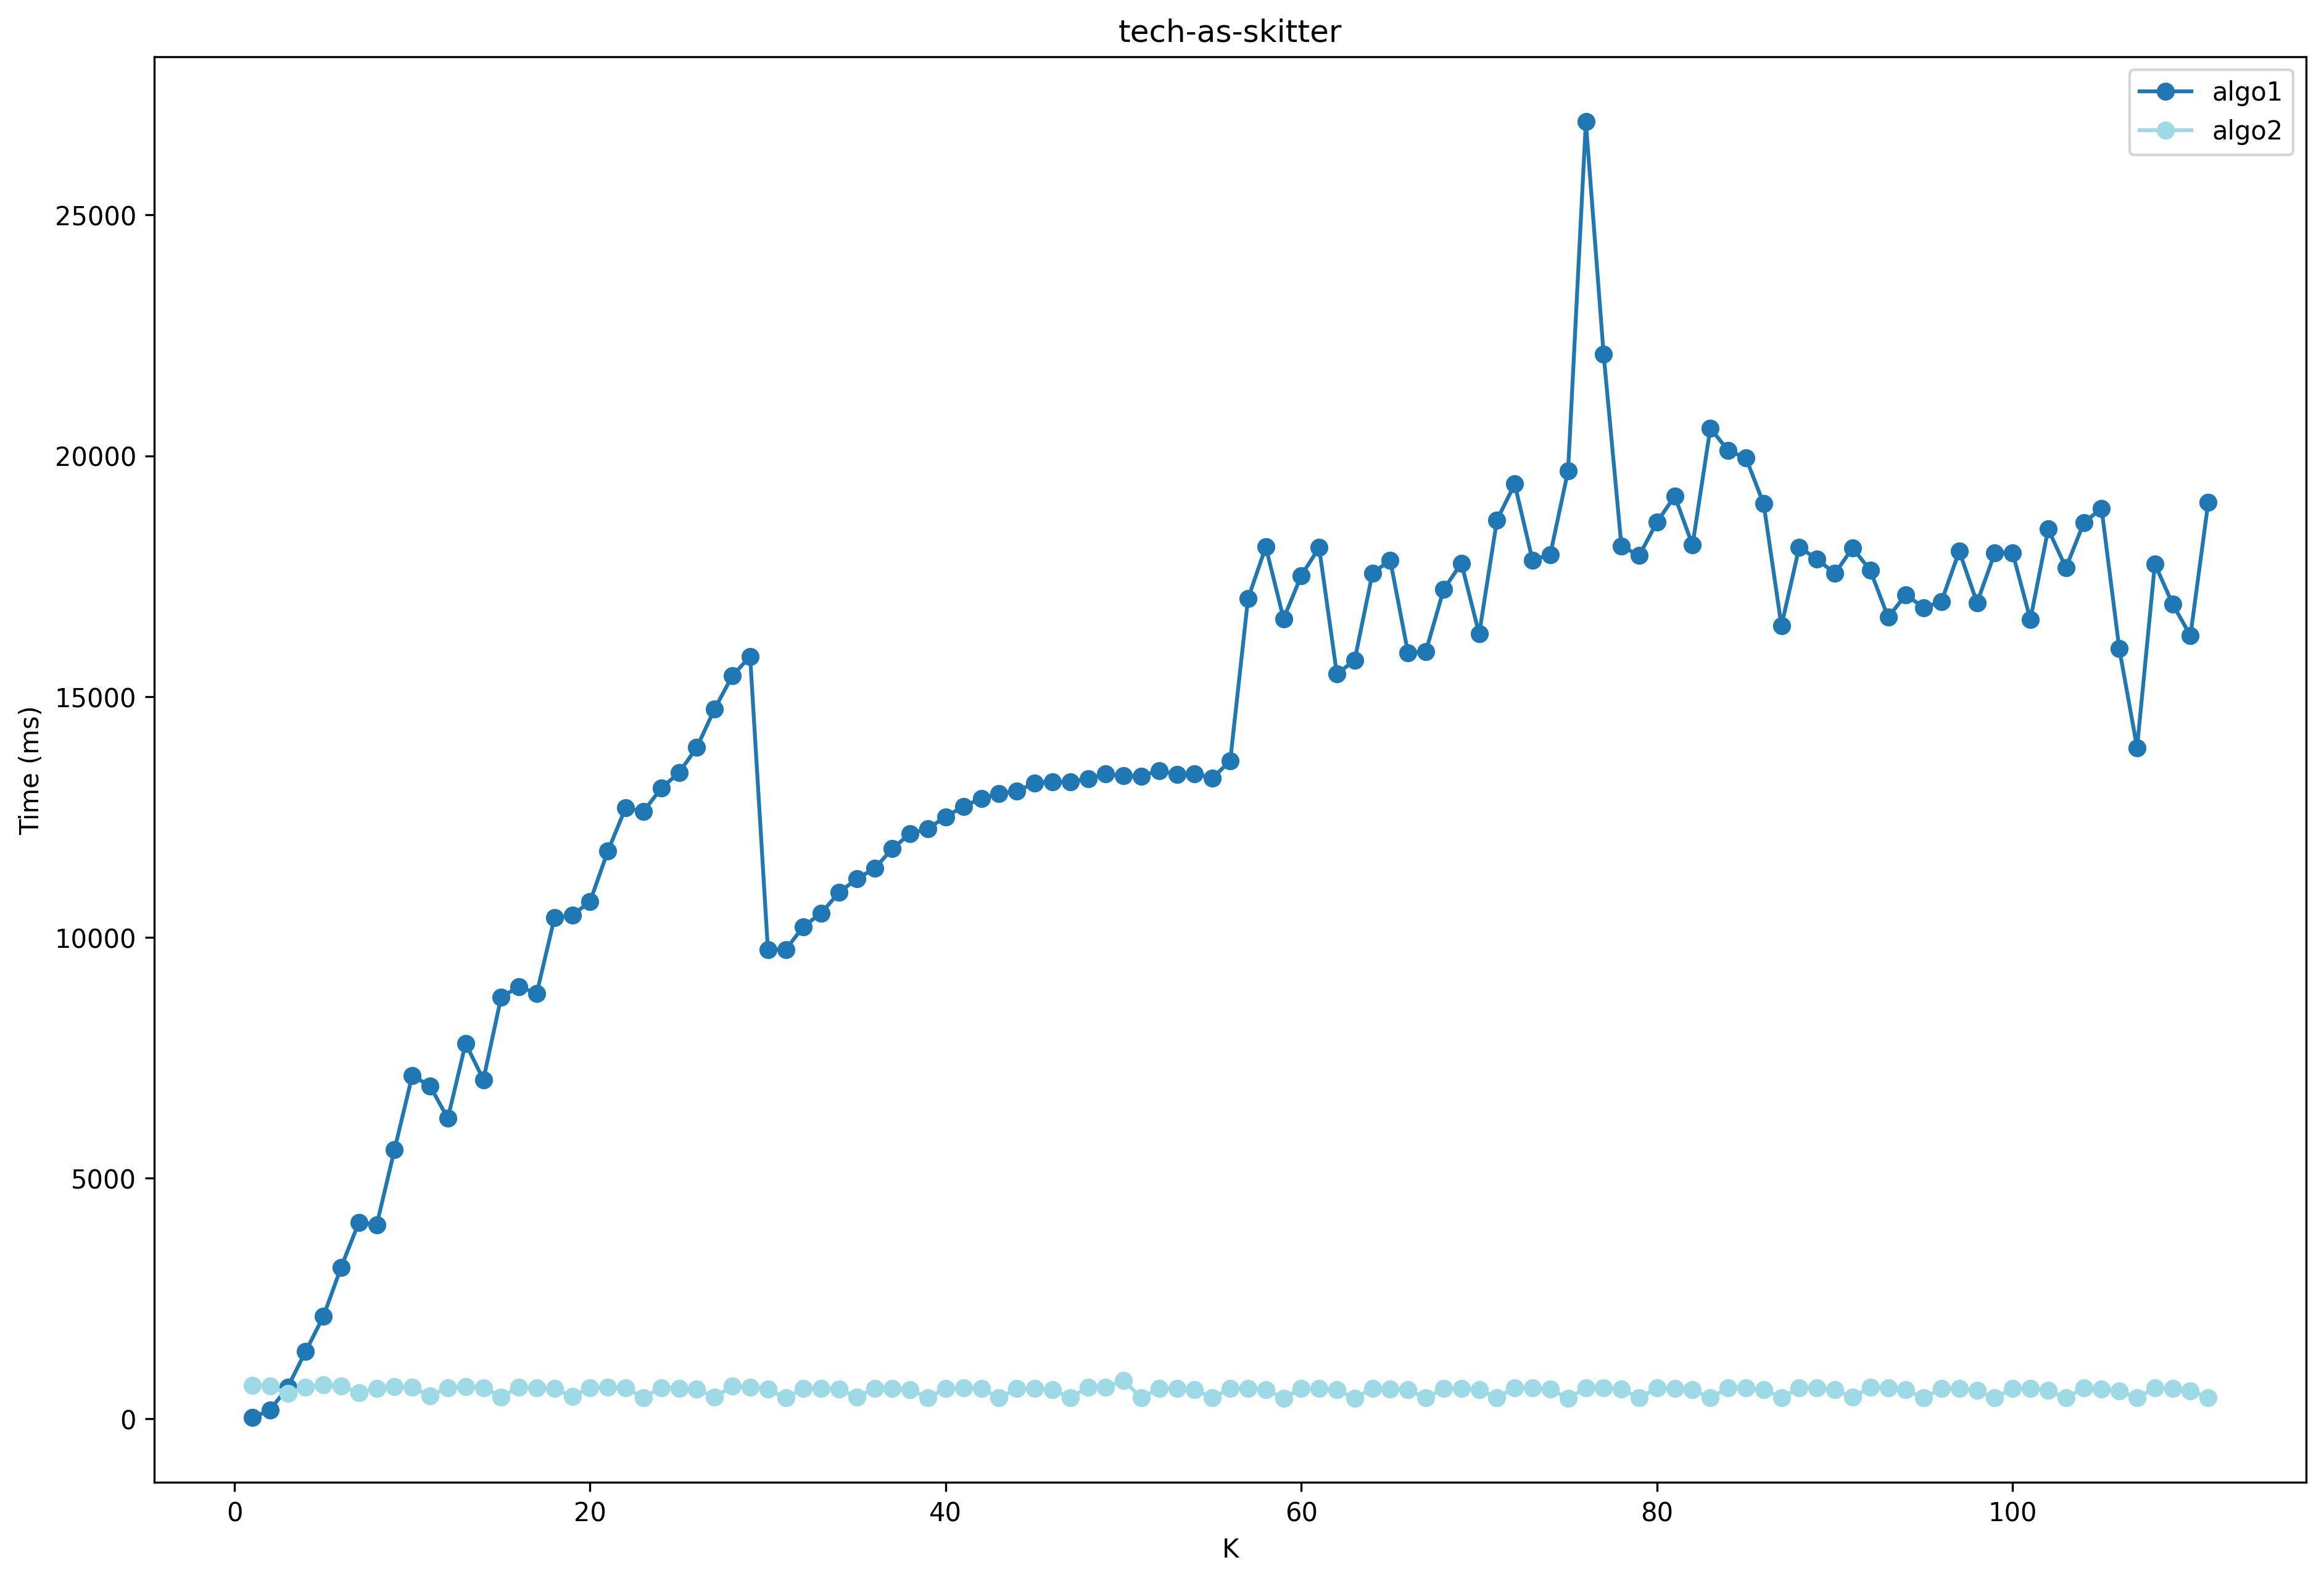
\includegraphics[width=0.6\textwidth]{Figures/tech-as-skitter.png}
    \caption{tech-as-skitter benchmark times for both algorithms}
    \label{fig:tech-as-skitter}
\end{figure}

\begin{figure}[H]
    \centering
    \includegraphics[width=0.6\textwidth]{Figures/web-Google.png}
    \caption{web-Google benchmark times for both algorithms}
    \label{fig:web-google}
\end{figure}

\begin{figure}[H]
    \centering
    \includegraphics[width=0.6\textwidth]{Figures/WikiTalk.png}
    \caption{WikiTalk benchmark times for both algorithms}
    \label{fig:wikitalk}
\end{figure}